\setstretch{1.8}
\chapter{Results} % Write in your own chapter title
\label{Chapter5}
\lhead{Chapter 5. \emph{Results}} % Write in your own chapter title to set the page header

This chapter shows the results for the tests performed. The tests were performed on 1 hp and 1.5 hp motors, both rated for 220V and 50Hz.

\clearpage
\section{1 hp Motor}
\subsection{Motor characteristics}

\begin{figure}[hbtp!]
	\centering
		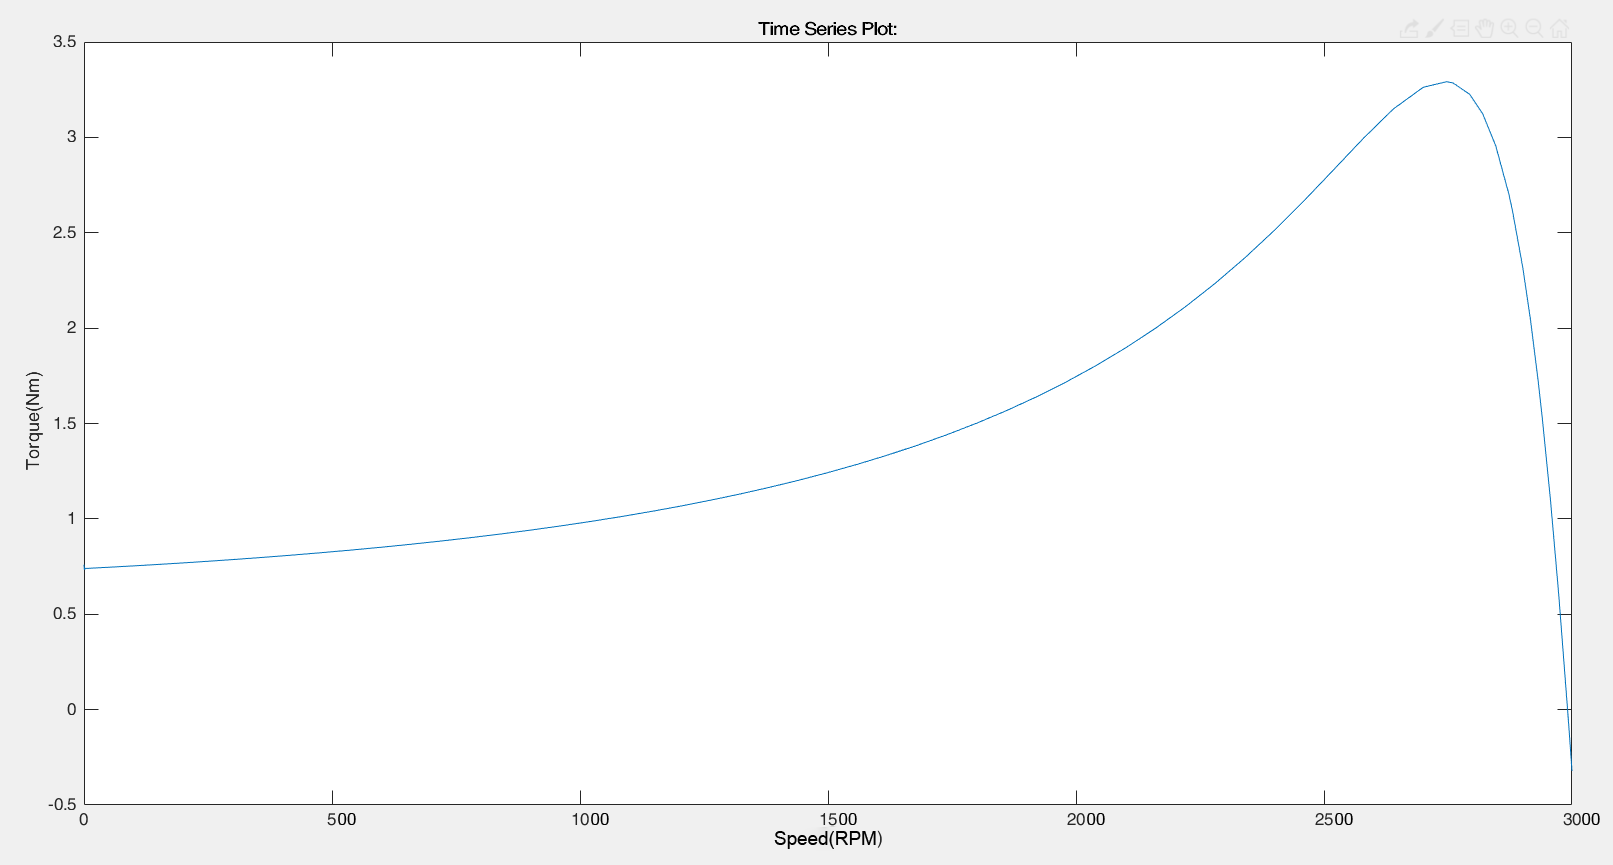
\includegraphics[width = 4.5in]{./Figures/MS/fig51.png}
		\rule{35em}{0.5pt}
	\caption{1hp motor torque-speed characteristics}
	\label{fig:1hp motor torque-speed characteristics} 
\end{figure}

\begin{figure}[hbtp!]
	\centering
		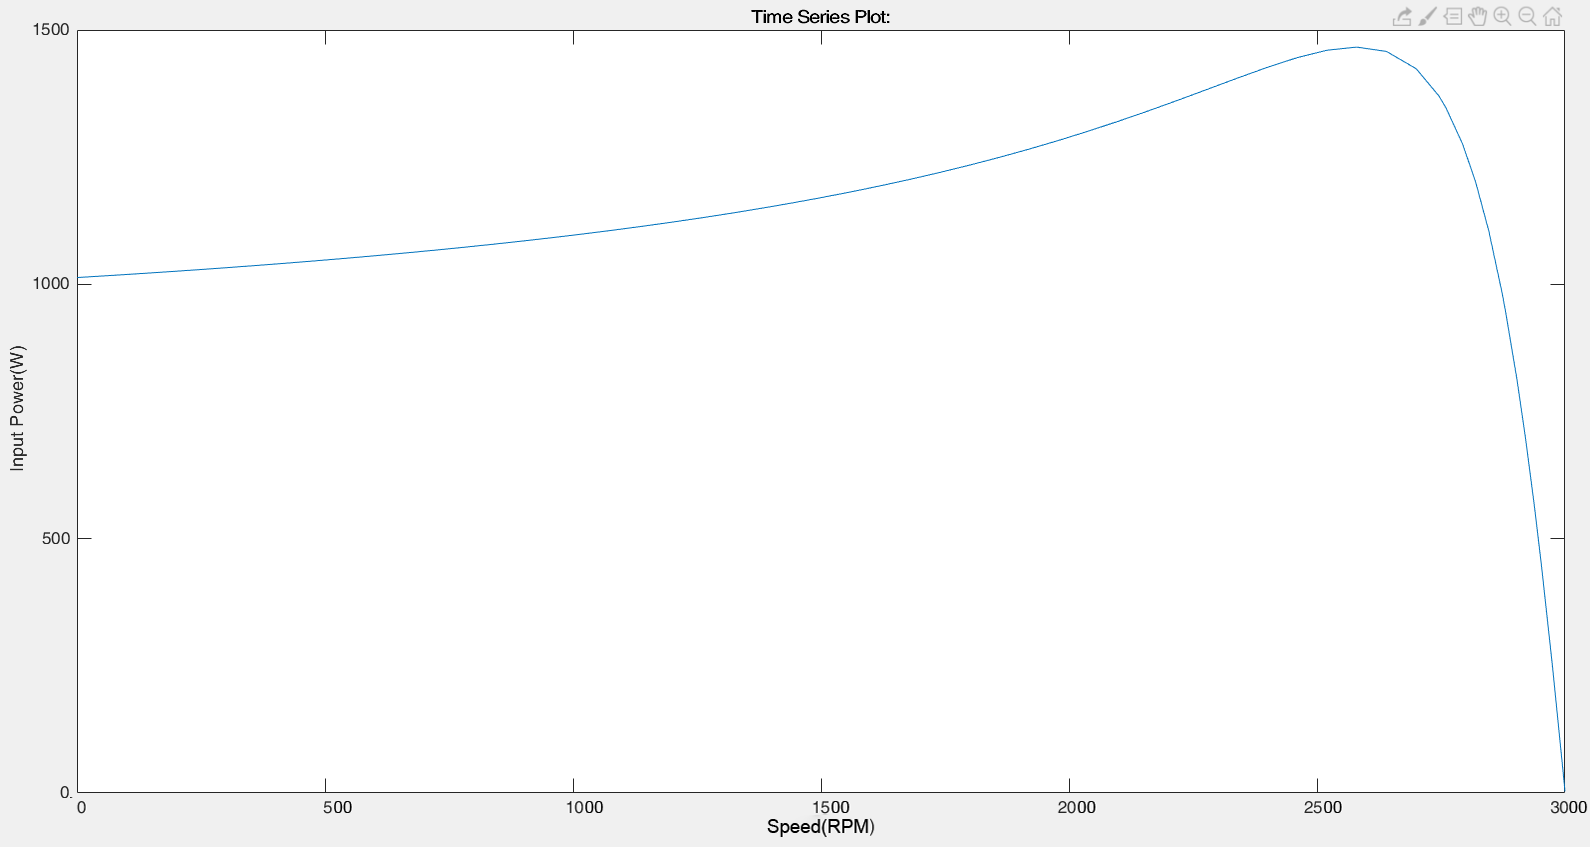
\includegraphics[width = 4.5in]{./Figures/MS/fig52.png}
		\rule{35em}{0.5pt}
	\caption{1hp motor input power characteristics}
	\label{fig:1hp motor input power characteristics} 
\end{figure}

\begin{figure}[hbtp!]
	\centering
		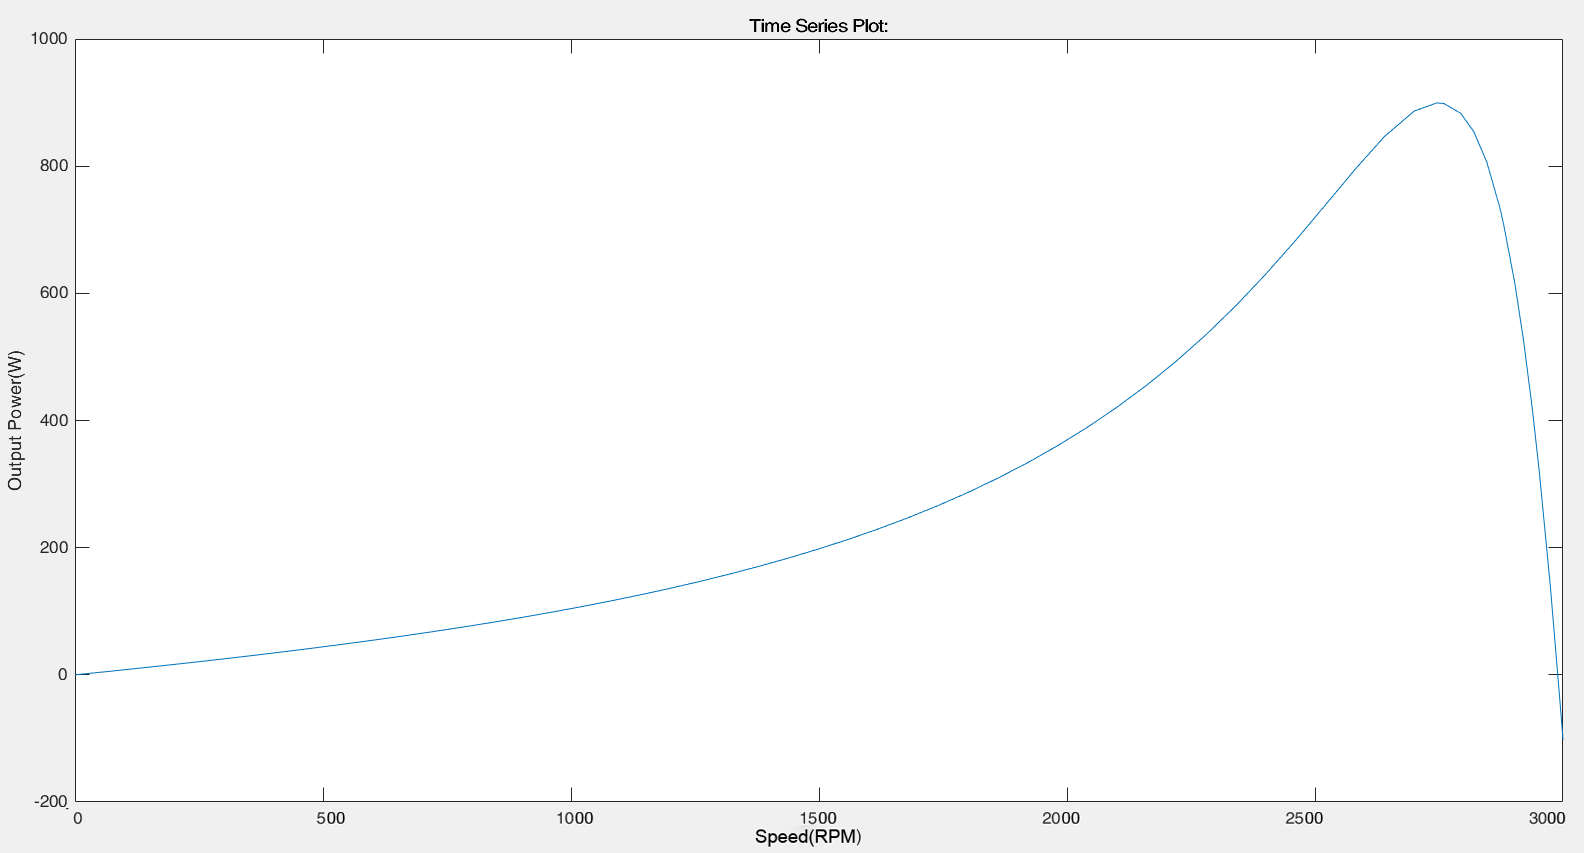
\includegraphics[width = 4.5in]{./Figures/MS/fig53.png}
		\rule{35em}{0.5pt}
	\caption{1hp motor output power characteristics}
	\label{fig:1hp motor output power characteristics} 
\end{figure}

\clearpage
\subsection{Method 1}
\subsubsection{Rated Load Test}
Following table shows the test results:
\begin{table}[hbtp!]
\begin{tabular}{>{\columncolor[HTML]{9B9B9B}}l llll}
    \cellcolor[HTML]{656565}{\color[HTML]{000000} Name} & \cellcolor[HTML]{656565}Symbol            & \cellcolor[HTML]{656565}Value     & \cellcolor[HTML]{656565}Unit &  \\
    {\color[HTML]{000000} Current}                      & I                                         & 4.7054                            & A                            &  \\
    {\color[HTML]{000000} Input   Power}                & \cellcolor[HTML]{F2F2F2}P1                & \cellcolor[HTML]{F2F2F2}978.26    & \cellcolor[HTML]{F2F2F2}W    &  \\
    {\color[HTML]{000000} Speed}                        & w                                         & 303.5737                          & rad/s                        &  \\
    {\color[HTML]{000000} Torque}                       & \cellcolor[HTML]{F2F2F2}T                 & \cellcolor[HTML]{F2F2F2}2.4574    & \cellcolor[HTML]{F2F2F2}Nm   &  \\
    {\color[HTML]{000000} stator resistance}            & R1                                        & 3.9                               & ohm                          &  \\
    {\color[HTML]{000000} slip}                         & \cellcolor[HTML]{F2F2F2}s                 & \cellcolor[HTML]{F2F2F2}0.0332    & \cellcolor[HTML]{F2F2F2}     &  \\
    {\color[HTML]{000000} Output   Power}               & P2                                        & 746.00201                         & W                            &  \\
    efficiency                                          & \cellcolor[HTML]{F2F2F2}P2/P1*100         & \cellcolor[HTML]{F2F2F2}76.25805  & \cellcolor[HTML]{F2F2F2}\%   &  \\
    Actual   losses                                     & P1-P2                                     & 232.25799                         & W                            &  \\
    Stator   Copper Loss                                & \cellcolor[HTML]{F2F2F2}Ps                & \cellcolor[HTML]{F2F2F2}86.34908  & \cellcolor[HTML]{F2F2F2}W    &  \\
    Rotor   Copper Loss                                 & Pr                                        & 26.68672                          & W                            &  \\
    Temp   correction factor                            & \cellcolor[HTML]{F2F2F2}k                 & \cellcolor[HTML]{F2F2F2}0.99631   & \cellcolor[HTML]{F2F2F2}     &  \\
    Temp corrected   slip                               & sc                                        & 0.03308                           &                              &  \\
    Temp   corrected Stator copper loss                 & \cellcolor[HTML]{F2F2F2}Ps,c              & \cellcolor[HTML]{F2F2F2}86.34908  & \cellcolor[HTML]{F2F2F2}W    &  \\
    Temp   corrected Rotor copper loss                  & Pr,c                                      & 26.58827                          & W                            &  \\
    Iron Loss                                           & \cellcolor[HTML]{F2F2F2}Pfe               & \cellcolor[HTML]{F2F2F2}88.20973  & \cellcolor[HTML]{F2F2F2}W    &  \\
    Friction\&Windage   Loss                            & Pfw                                       & 10.22740                          & W                            &  \\
    Calculated   Losses                                 & \cellcolor[HTML]{F2F2F2}Ps,c+Pr,c+Pfe+Pfw & \cellcolor[HTML]{F2F2F2}211.37448 & \cellcolor[HTML]{F2F2F2}W    &  \\
    Residual   Losses                                   & P\_Lr                                     & 20.88351                          & W                            & 
\end{tabular}
\end{table}

\subsubsection{Load curve test}
Following table shows the test results:
\begin{table}[hbtp!]
\begin{tabular}{lllllll}
    \rowcolor[HTML]{343434} 
    Load   points                                & 125\%    & 115\%    & 100\%    & 75\%     & 50\%     & 25\%     \\
    \rowcolor[HTML]{F2F2F2} 
    \cellcolor[HTML]{9B9B9B}Input   Power        & 1443.1   & 1171     & 978.26   & 722.1448 & 499.2    & 293.46   \\
    \cellcolor[HTML]{9B9B9B}Current              & 7.8101   & 5.8201   & 4.7054   & 3.3768   & 2.2977   & 1.3397   \\
    \rowcolor[HTML]{F2F2F2} 
    \cellcolor[HTML]{9B9B9B}Speed                & 289.0265 & 299.4447 & 303.5737 & 307.472  & 310.0261 & 311.9381 \\
    \cellcolor[HTML]{9B9B9B}Torque               & 3.2327   & 2.865    & 2.4574   & 1.8197   & 1.2031   & 0.5979   \\
    \rowcolor[HTML]{F2F2F2} 
    \cellcolor[HTML]{9B9B9B}slip                 & 0.0795   & 0.0464   & 0.0332   & 0.0208   & 0.0127   & 0.0066   \\
    \cellcolor[HTML]{9B9B9B}Output   Power       & 934.3360 & 857.9091 & 746.0020 & 559.5068 & 372.9924 & 186.5078 \\
    \rowcolor[HTML]{F2F2F2} 
    \cellcolor[HTML]{9B9B9B}Actual   Losses      & 508.7640 & 313.0909 & 232.2580 & 162.6380 & 126.2076 & 106.9522 \\
    \cellcolor[HTML]{9B9B9B}Efficiency           & 64.7451  & 73.2629  & 76.2581  & 77.4785  & 74.7180  & 63.5548  \\
    \rowcolor[HTML]{F2F2F2} 
    \cellcolor[HTML]{9B9B9B}Stator   Copper Loss & 237.8909 & 132.1069 & 86.3491  & 44.4708  & 20.5898  & 6.9997   \\
    \cellcolor[HTML]{9B9B9B}Rotor   Copper Loss  & 88.8388  & 44.0684  & 26.6867  & 12.2548  & 4.9408   & 1.3018   \\
    \rowcolor[HTML]{F2F2F2} 
    \cellcolor[HTML]{9B9B9B}Calculated   Losses  & 425.1668 & 274.6124 & 211.4729 & 155.1628 & 123.9677 & 106.7387 \\
    \cellcolor[HTML]{9B9B9B}P\_lr                & 83.5972  & 38.4785  & 20.7851  & 7.4752   & 2.2399   & 0.2136  
\end{tabular}
\end{table}

\subsubsection{No load test}
Following table shows the test results:
\begin{table}[hbtp!]
\begin{tabular}{llll}
    \rowcolor[HTML]{656565} 
    Name                                                              & Symbol  & Value    & Unit  \\
    \cellcolor[HTML]{656565}Voltage                                   & V\_0    & 220      & V     \\
    \rowcolor[HTML]{F2F2F2} 
    \cellcolor[HTML]{656565}Current                                   & I\_0    & 1.5107   & A     \\
    \cellcolor[HTML]{656565}Input   Power                             & P\_0    & 106.4249 & W     \\
    \rowcolor[HTML]{F2F2F2} 
    \cellcolor[HTML]{656565}Stator   Copper Loss                      & P\_s\_0 & 7.9877   & W     \\
    \cellcolor[HTML]{656565}Speed at   rated power                    & n\_rl   & 303.5737 & rad/s \\
    \rowcolor[HTML]{F2F2F2} 
    \cellcolor[HTML]{656565}Torque   Req. to rotate unenergized motor & T\_0    & 0.0307   & Nm    \\
    \cellcolor[HTML]{656565}Friction\&Windage   Loss                  & P\_fw   & 10.2274  & W     \\
    \rowcolor[HTML]{F2F2F2} 
    \cellcolor[HTML]{656565}Iron Loss                                 & P\_fe   & 88.2097  & W    
\end{tabular}
\end{table}

\begin{figure}[hbtp!]
	\centering
		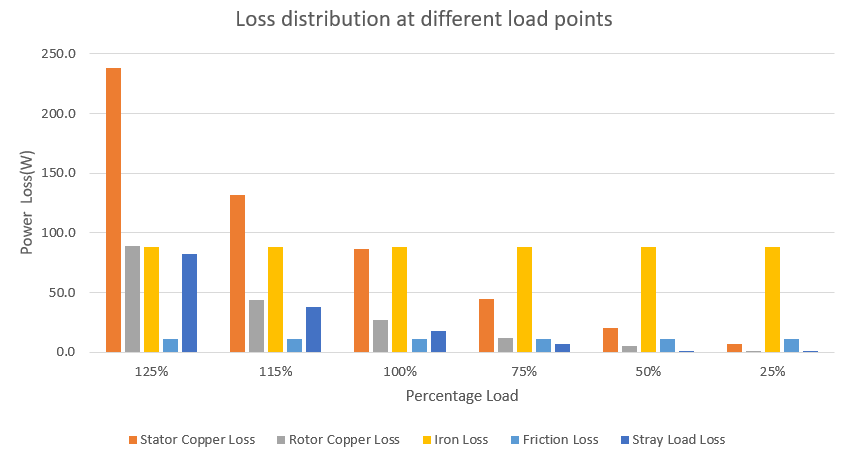
\includegraphics[width = 4.5in]{./Figures/MS/fig54.png}
		\rule{35em}{0.5pt}
	\caption{Bar graph for losses at different load points for 1hp motor(method1)}
	\label{fig:Bar graph for losses at different load points for 1hp motor(method1)} 
\end{figure}

\begin{figure}[hbtp!]
	\centering
		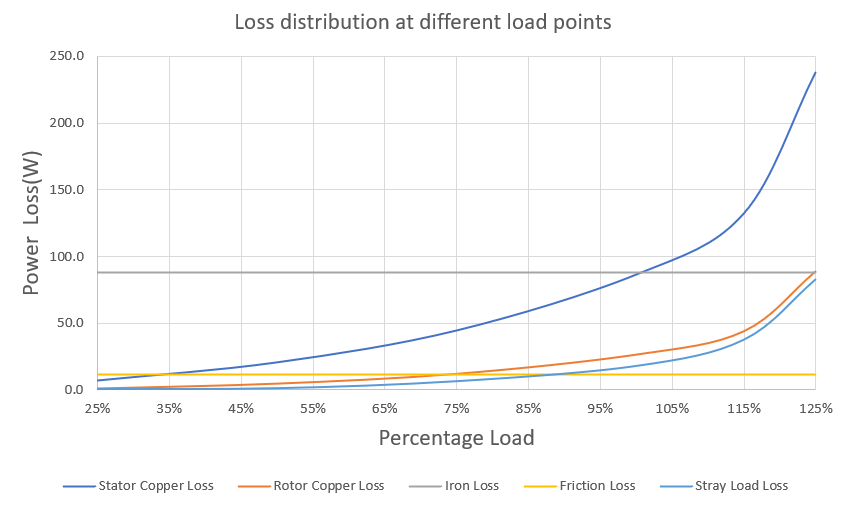
\includegraphics[width = 4.5in]{./Figures/MS/fig55.png}
		\rule{35em}{0.5pt}
	\caption{Line chart for losses at different load points for 1hp motor(method1)}
	\label{fig:Line chart for losses at different load points for 1hp motor(method1)} 
\end{figure}

\begin{figure}[hbtp!]
	\centering
		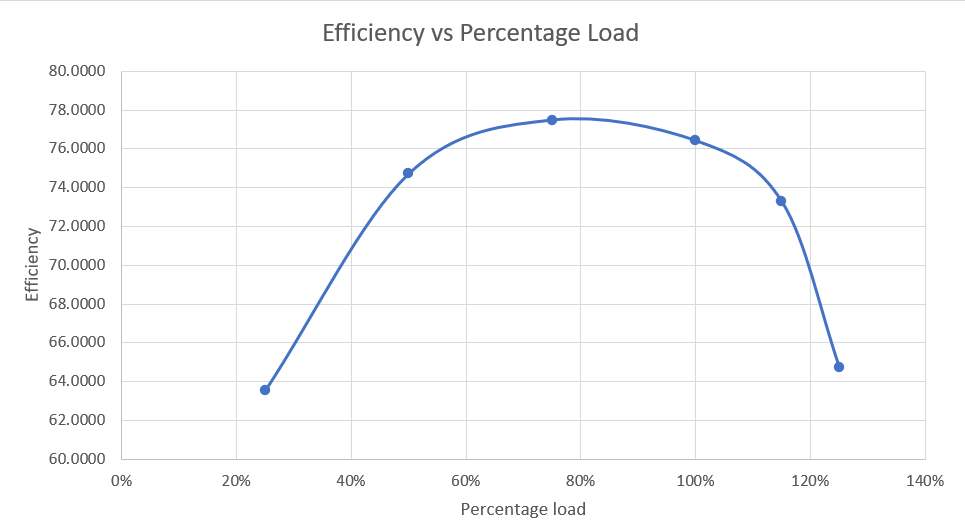
\includegraphics[width = 4.5in]{./Figures/MS/fig56.png}
		\rule{35em}{0.5pt}
	\caption{Percentage load vs efficiency for 1hp motor(method1)}
	\label{fig:Percentage load vs efficiency for 1hp motor(method1)} 
\end{figure}

\begin{figure}[hbtp!]
	\centering
		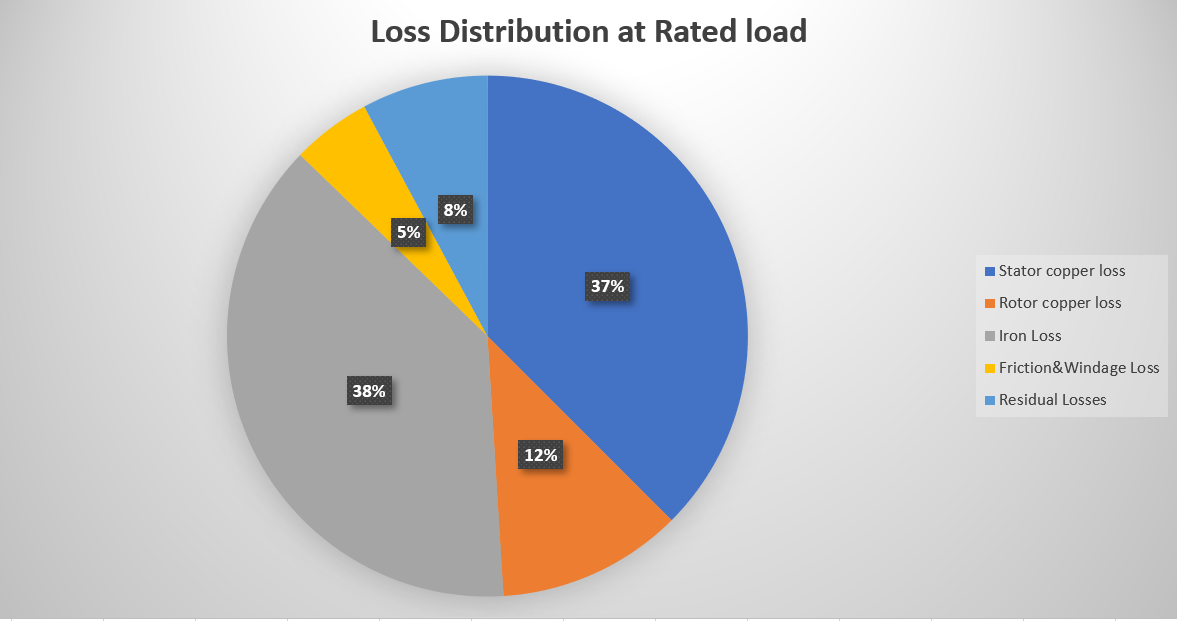
\includegraphics[width = 4.5in]{./Figures/MS/fig57.png}
		\rule{35em}{0.5pt}
	\caption{Pie chart for loss distribution at rated load for 1hp motor(method1)}
	\label{fig:Pie chart for loss distribution at rated load for 1hp motor(method1)} 
\end{figure}

\clearpage
\subsection{Method 2}
\subsubsection{Rated Load Test}
Following table shows the test results:
\begin{table}[hbtp!]
\begin{tabular}{
    >{\columncolor[HTML]{9B9B9B}}l llll}
    \cellcolor[HTML]{656565}{\color[HTML]{000000} Name} & \cellcolor[HTML]{656565}Symbol            & \cellcolor[HTML]{656565}Value     & \cellcolor[HTML]{656565}Unit &  \\
    {\color[HTML]{000000} Current}                      & I                                         & 4.7048                            & A                            &  \\
    {\color[HTML]{000000} Input   Power}                & \cellcolor[HTML]{F2F2F2}P1                & \cellcolor[HTML]{F2F2F2}978.13    & \cellcolor[HTML]{F2F2F2}W    &  \\
    {\color[HTML]{000000} Speed}                        & w                                         & 303.6252                          & rad/s                        &  \\
    {\color[HTML]{000000} Torque}                       & \cellcolor[HTML]{F2F2F2}T                 & \cellcolor[HTML]{F2F2F2}2.4569    & \cellcolor[HTML]{F2F2F2}Nm   &  \\
    {\color[HTML]{000000} stator   resistance}          & R1                                        & 3.9                               & ohm                          &  \\
    {\color[HTML]{000000} slip}                         & \cellcolor[HTML]{F2F2F2}s                 & \cellcolor[HTML]{F2F2F2}0.0330    & \cellcolor[HTML]{F2F2F2}     &  \\
    {\color[HTML]{000000} Output   Power}               & P2                                        & 745.97675                         & W                            &  \\
    efficiency                                          & \cellcolor[HTML]{F2F2F2}P2/P1*100         & \cellcolor[HTML]{F2F2F2}76.26560  & \cellcolor[HTML]{F2F2F2}\%   &  \\
    Actual   losses                                     & P1-P2                                     & 232.15325                         & W                            &  \\
    Stator   Copper Loss                                & \cellcolor[HTML]{F2F2F2}Ps                & \cellcolor[HTML]{F2F2F2}86.32706  & \cellcolor[HTML]{F2F2F2}W    &  \\
    Rotor   Copper Loss                                 & Pr                                        & 26.55133                          & W                            &  \\
    Temp   correction factor                            & \cellcolor[HTML]{F2F2F2}k                 & \cellcolor[HTML]{F2F2F2}0.99631   & \cellcolor[HTML]{F2F2F2}     &  \\
    Temp corrected   slip                               & sc                                        & 0.03292                           &                              &  \\
    Temp   corrected Stator copper loss                 & \cellcolor[HTML]{F2F2F2}Ps,c              & \cellcolor[HTML]{F2F2F2}86.32706  & \cellcolor[HTML]{F2F2F2}W    &  \\
    Temp   corrected Rotor copper loss                  & Pr,c                                      & 26.45339                          & W                            &  \\
    Iron Loss                                           & \cellcolor[HTML]{F2F2F2}Pfe               & \cellcolor[HTML]{F2F2F2}88.20973  & \cellcolor[HTML]{F2F2F2}W    &  \\
    Friction\&Windage   Loss                            & Pfw                                       & 10.22740                          & W                            &  \\
    Calculated   Losses                                 & \cellcolor[HTML]{F2F2F2}Ps,c+Pr,c+Pfe+Pfw & \cellcolor[HTML]{F2F2F2}211.21757 & \cellcolor[HTML]{F2F2F2}W    &  \\
    Residual   Losses                                   & P\_Lr                                     & 20.93567                          & W                            & 
\end{tabular}
\end{table}

\subsubsection{Load curve test}
Following table shows the test results:
\begin{table}[hbtp!]
\begin{tabular}{lllllll}
    \rowcolor[HTML]{343434} 
    Load   points                                & 125\%    & 115\%    & 100\%    & 75\%     & 50\%     & 25\%     \\
    \rowcolor[HTML]{F2F2F2} 
    \cellcolor[HTML]{656565}Input   Power        & 1443.5   & 1171.1   & 978.13   & 722.1448 & 499.2    & 293.46   \\
    \cellcolor[HTML]{656565}Current              & 7.8095   & 5.8321   & 4.7048   & 3.3658   & 2.2795   & 1.3352   \\
    \rowcolor[HTML]{F2F2F2} 
    \cellcolor[HTML]{656565}Speed                & 289.0524 & 299.4647 & 303.6252 & 307.435  & 310.0315 & 311.9522 \\
    \cellcolor[HTML]{656565}Torque               & 3.233    & 2.862    & 2.4569   & 1.8191   & 1.2037   & 0.5976   \\
    \rowcolor[HTML]{F2F2F2} 
    \cellcolor[HTML]{656565}slip                 & 0.0795   & 0.0463   & 0.0330   & 0.0209   & 0.0126   & 0.0065   \\
    \cellcolor[HTML]{656565}Output   Power       & 934.5064 & 857.0680 & 745.9768 & 559.2550 & 373.1849 & 186.4226 \\
    \rowcolor[HTML]{F2F2F2} 
    \cellcolor[HTML]{656565}Actual   Losses      & 508.9936 & 314.0320 & 232.1532 & 162.8898 & 126.0151 & 107.0374 \\
    \cellcolor[HTML]{656565}Efficiency           & 64.7389  & 73.1849  & 76.2656  & 77.4436  & 74.7566  & 63.5257  \\
    \rowcolor[HTML]{F2F2F2} 
    \cellcolor[HTML]{656565}Stator   Copper Loss & 237.8543 & 132.6522 & 86.3271  & 44.1816  & 20.2649  & 6.9528   \\
    \cellcolor[HTML]{656565}Rotor   Copper Loss  & 88.7814  & 43.9872  & 26.5513  & 12.3304  & 4.9382   & 1.2932   \\
    \rowcolor[HTML]{F2F2F2} 
    \cellcolor[HTML]{656565}Calculated   Losses  & 425.0728 & 275.0766 & 211.3155 & 154.9491 & 123.6402 & 106.6831 \\
    \cellcolor[HTML]{656565}P\_lr                & 83.9208  & 38.9554  & 20.8377  & 7.9407   & 2.3749   & 0.3543   
\end{tabular}
\end{table}

\subsubsection{No load test}
Following table shows the test results:
\begin{table}[hbtp!]
\begin{tabular}{llll}
    \rowcolor[HTML]{656565} 
    Name                                                              & Symbol  & Value    & Unit  \\
    \cellcolor[HTML]{656565}Voltage                                 & V\_0    & 220      & V       \\
    \rowcolor[HTML]{F2F2F2} 
    \cellcolor[HTML]{656565}Current                                 & I\_0    & 1.5107   & A       \\
    \cellcolor[HTML]{656565}Input Power                             & P\_0    & 106.4249 & W       \\
    \rowcolor[HTML]{F2F2F2} 
    \cellcolor[HTML]{656565}Stator Copper Loss                      & P\_s\_0 & 7.9877   & W       \\
    \cellcolor[HTML]{656565}Speed at rated power                    & n\_rl   & 303.6252 & rad/s   \\
    \rowcolor[HTML]{F2F2F2} 
    \cellcolor[HTML]{656565}Torque Req. to rotate unenergized motor & T\_0    & 0.0307   & Nm      \\
    \cellcolor[HTML]{656565}Friction\&Windage Loss                  & P\_fw   & 10.2274  & W       \\
    \rowcolor[HTML]{F2F2F2} 
    \cellcolor[HTML]{656565}Iron Loss                               & P\_fe   & 88.2097  & W      
\end{tabular}
\end{table}

\begin{figure}[hbtp!]
	\centering
		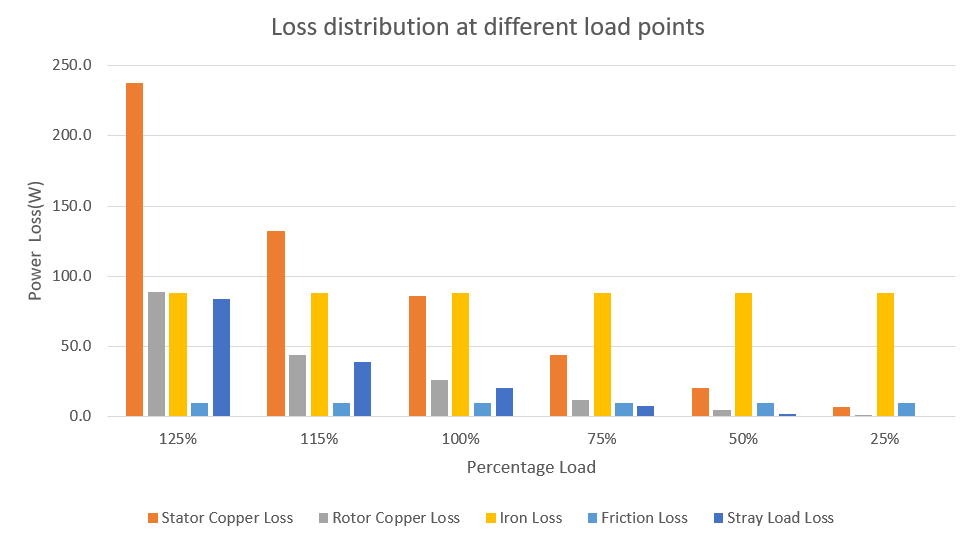
\includegraphics[width = 4.5in]{./Figures/MS/fig58.png}
		\rule{35em}{0.5pt}
	\caption{Bar graph for losses at different load points for 1hp motor(method2)}
	\label{fig:Bar graph for losses at different load points for 1hp motor(method2)} 
\end{figure}

\begin{figure}[hbtp!]
	\centering
		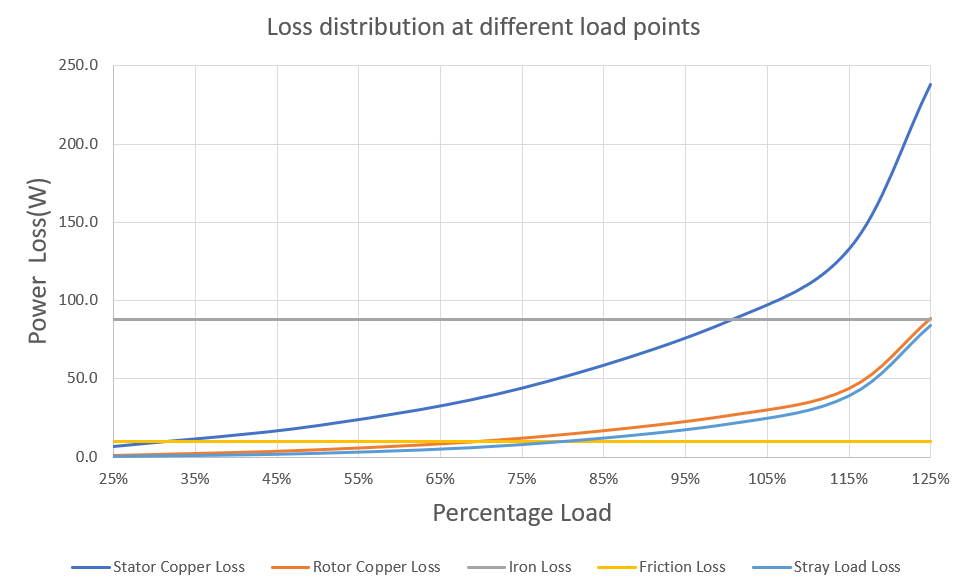
\includegraphics[width = 4.5in]{./Figures/MS/fig59.png}
		\rule{35em}{0.5pt}
	\caption{Line chart for losses at different load points for 1hp motor(method2)}
	\label{fig:Line chart for losses at different load points for 1hp motor(method2)} 
\end{figure}

\begin{figure}[hbtp!]
	\centering
		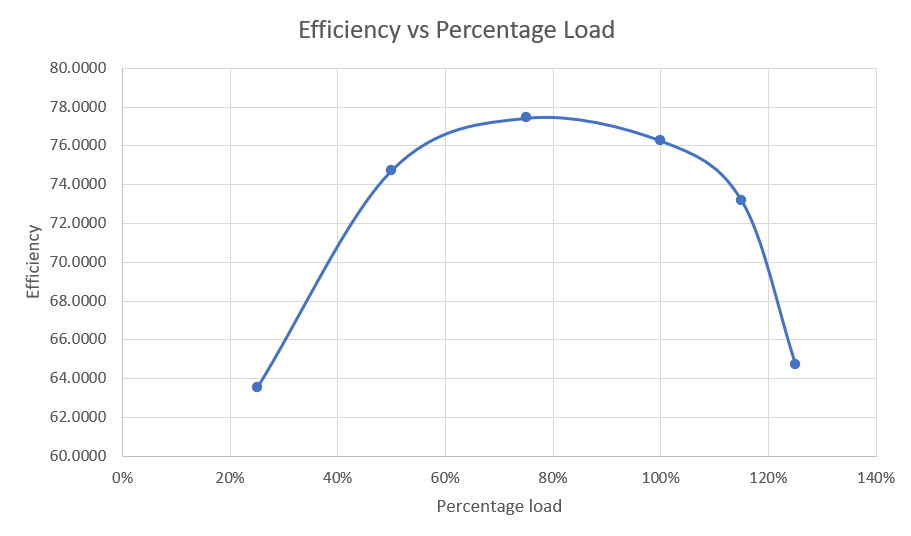
\includegraphics[width = 4.5in]{./Figures/MS/fig510.png}
		\rule{35em}{0.5pt}
	\caption{Percentage load vs efficiency for 1hp motor(method2)}
	\label{fig:Percentage load vs efficiency for 1hp motor(method2)} 
\end{figure}

\begin{figure}[hbtp!]
	\centering
		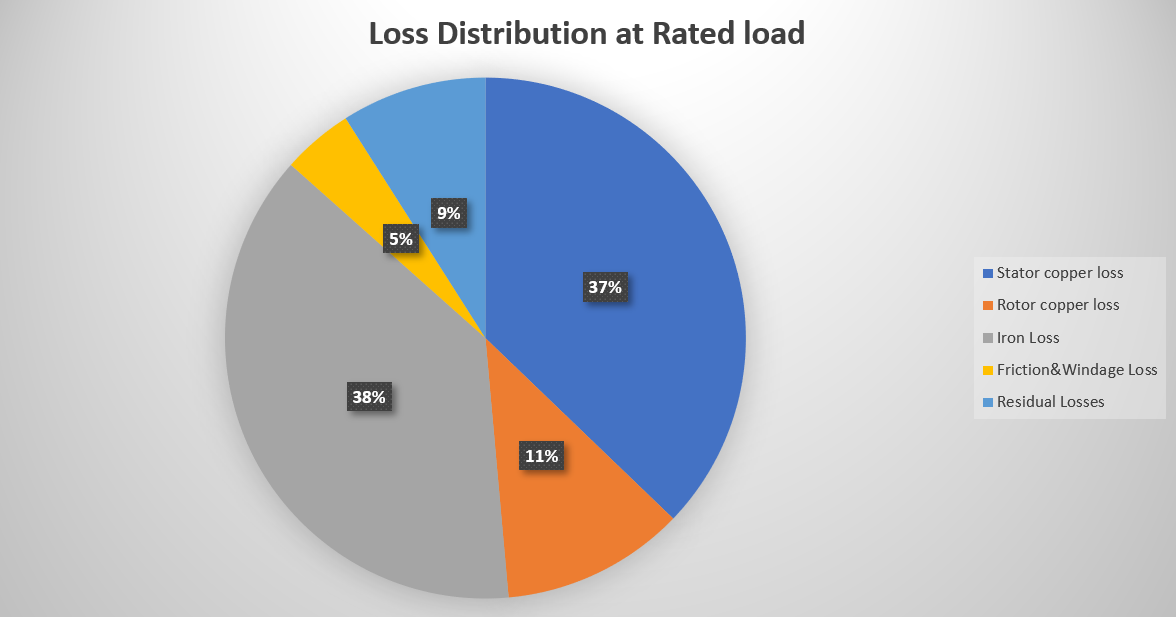
\includegraphics[width = 4.5in]{./Figures/MS/fig511.png}
		\rule{35em}{0.5pt}
	\caption{Pie chart for loss distribution at rated load for 1hp motor(method2)}
	\label{fig:Pie chart for loss distribution at rated load for 1hp motor(method2)} 
\end{figure}

\clearpage
\section{1.5 hp Motor}
\subsection{Motor characteristics}

\begin{figure}[hbtp!]
	\centering
		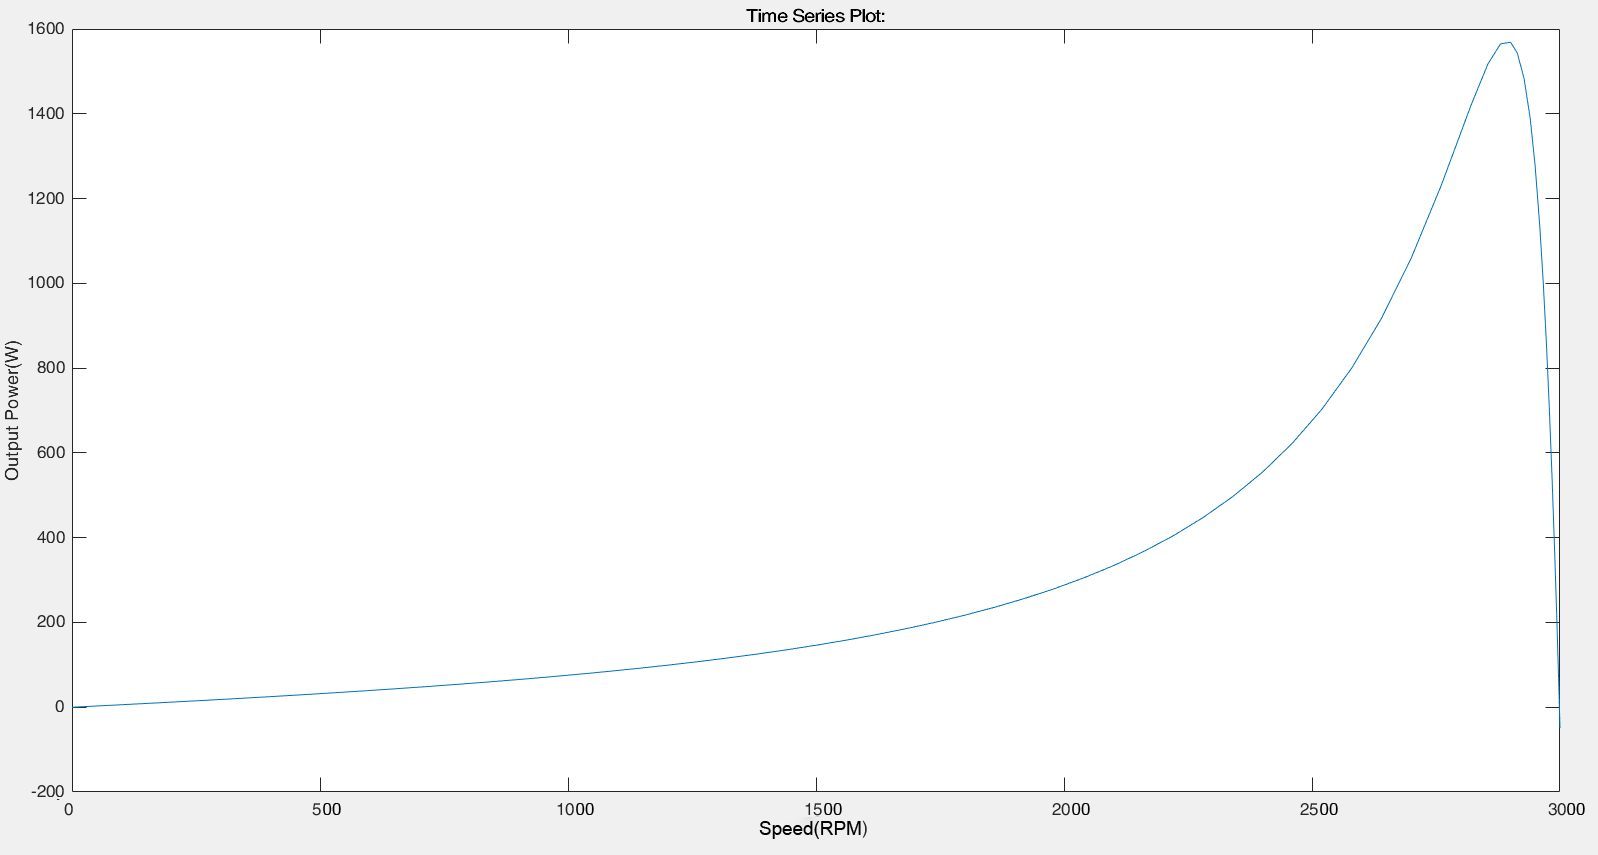
\includegraphics[width = 4.5in]{./Figures/MS/fig512.png}
		\rule{35em}{0.5pt}
	\caption{1.5 hp motor torque-speed characteristics}
	\label{fig:1.5 hp motor torque-speed characteristics} 
\end{figure}

\begin{figure}[hbtp!]
	\centering
		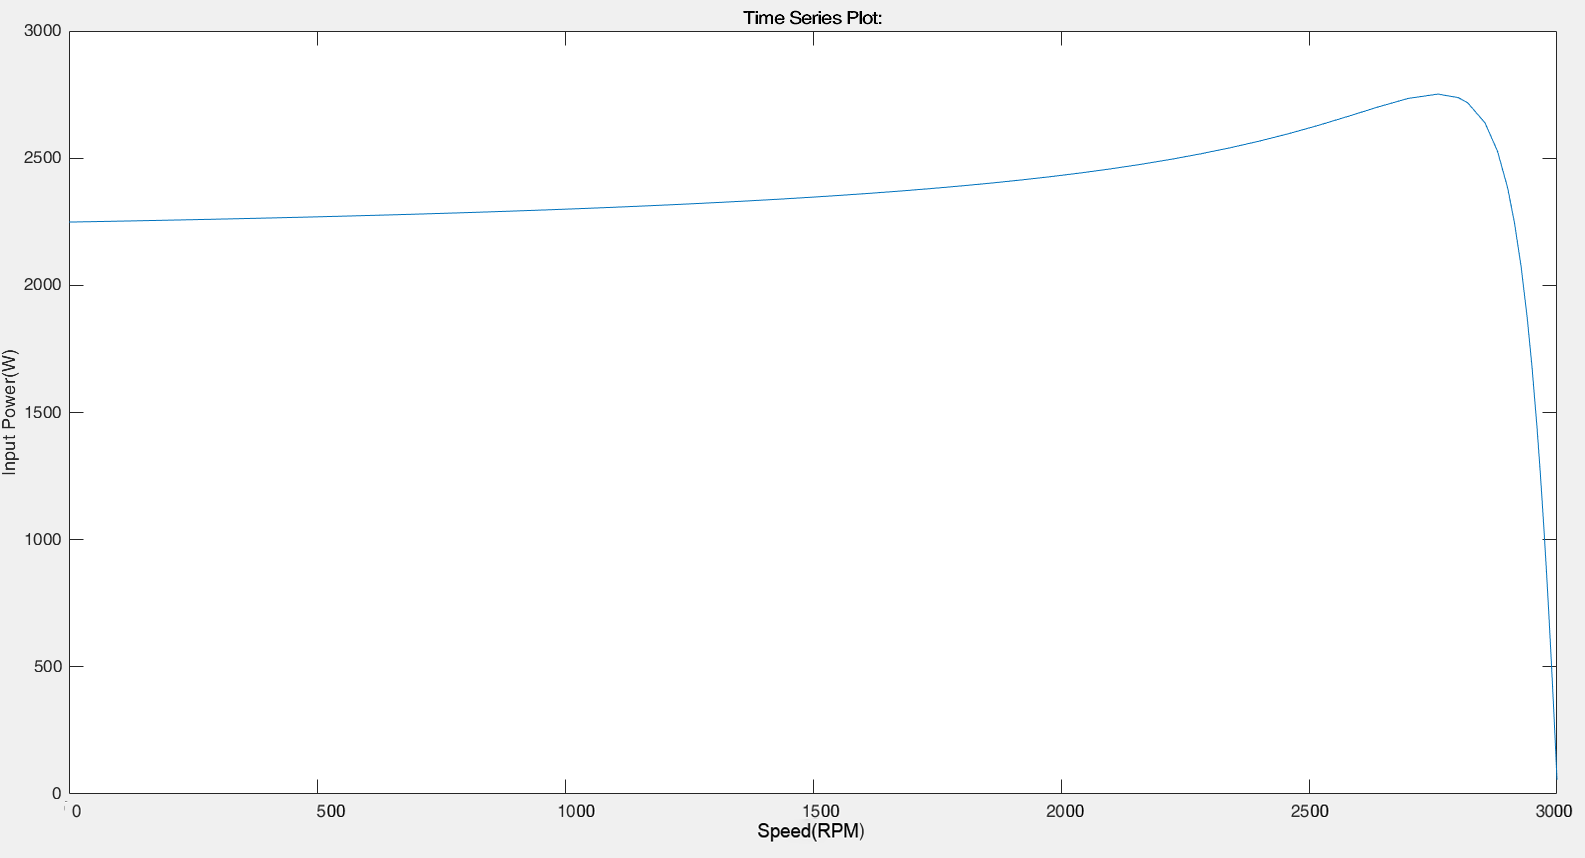
\includegraphics[width = 4.5in]{./Figures/MS/fig513.png}
		\rule{35em}{0.5pt}
	\caption{1.5 hp motor input power characteristics}
	\label{fig:1.5 hp motor input power characteristics} 
\end{figure}

\begin{figure}[hbtp!]
	\centering
		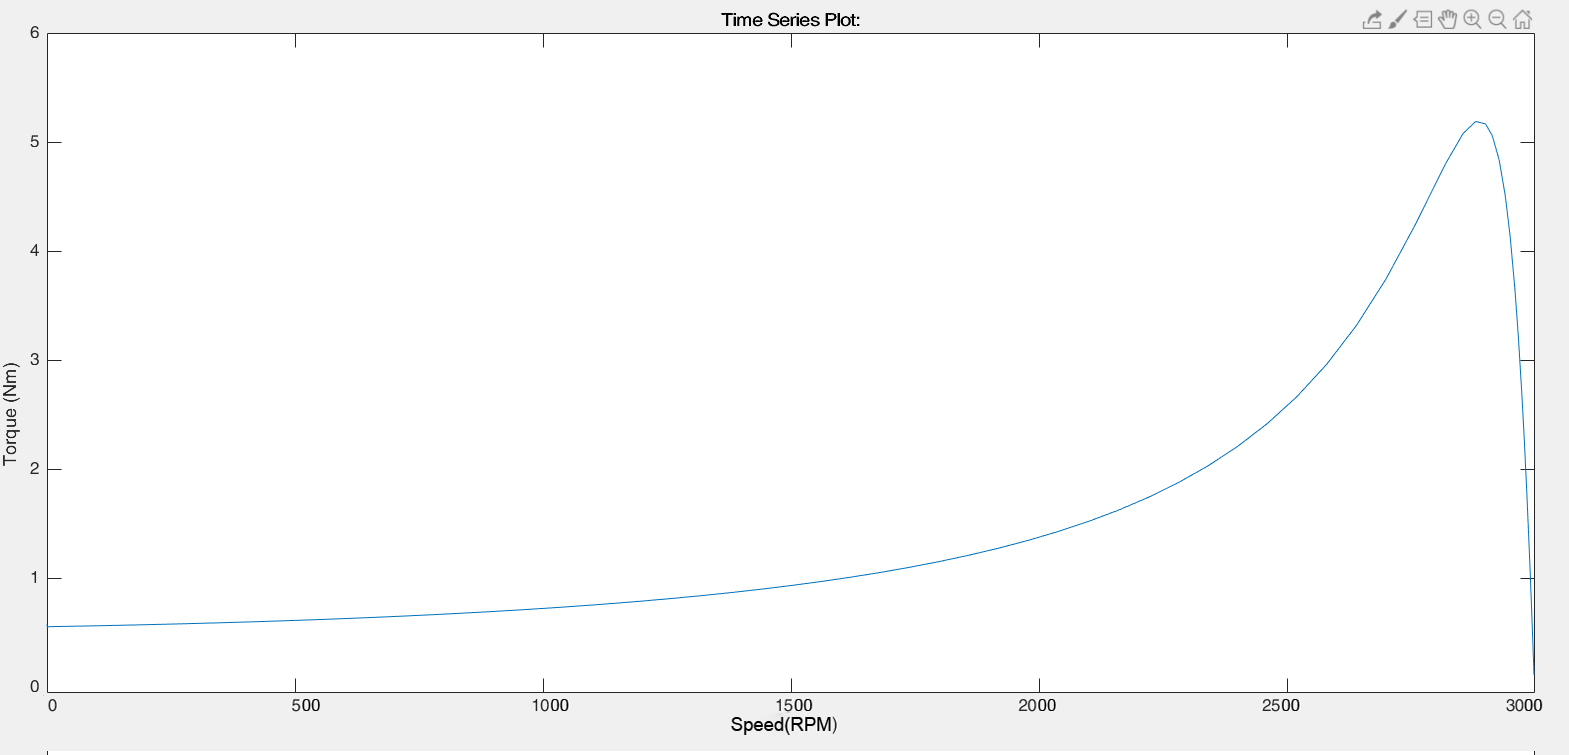
\includegraphics[width = 4.5in]{./Figures/MS/fig514.png}
		\rule{35em}{0.5pt}
	\caption{1.5 hp motor output power characteristics}
	\label{fig:1.5 hp motor output power characteristics} 
\end{figure}

\clearpage
\subsection{Method 1}
\subsubsection{Rated Load Test}
Following table shows the test results:
\begin{table}[hbtp!]
\begin{tabular}{
    >{\columncolor[HTML]{9B9B9B}}l llll}
    \cellcolor[HTML]{656565}{\color[HTML]{000000} Name} & \cellcolor[HTML]{656565}Symbol            & \cellcolor[HTML]{656565}Value     & \cellcolor[HTML]{656565}Unit &  \\
    {\color[HTML]{000000} Current}                      & I                                         & 7.0225                            & A                            &  \\
    {\color[HTML]{000000} Input   Power}                & \cellcolor[HTML]{F2F2F2}P1                & \cellcolor[HTML]{F2F2F2}1473.5    & \cellcolor[HTML]{F2F2F2}W    &  \\
    {\color[HTML]{000000} Speed}                        & w                                         & 309.8536                          & rad/s                        &  \\
    {\color[HTML]{000000} Torque}                       & \cellcolor[HTML]{F2F2F2}T                 & \cellcolor[HTML]{F2F2F2}3.6114    & \cellcolor[HTML]{F2F2F2}Nm   &  \\
    {\color[HTML]{000000} stator   resistance}          & R1                                        & 3.5                               & ohm                          &  \\
    {\color[HTML]{000000} slip}                         & \cellcolor[HTML]{F2F2F2}s                 & \cellcolor[HTML]{F2F2F2}0.0132    & \cellcolor[HTML]{F2F2F2}     &  \\
    {\color[HTML]{000000} Output   Power}               & P2                                        & 1119.00529                        & W                            &  \\
    efficiency                                          & \cellcolor[HTML]{F2F2F2}P2/P1*100         & \cellcolor[HTML]{F2F2F2}75.94199  & \cellcolor[HTML]{F2F2F2}\%   &  \\
    Actual   losses                                     & P1-P2                                     & 354.49471                         & W                            &  \\
    Stator   Copper Loss                                & \cellcolor[HTML]{F2F2F2}Ps                & \cellcolor[HTML]{F2F2F2}172.60427 & \cellcolor[HTML]{F2F2F2}W    &  \\
    Rotor   Copper Loss                                 & Pr                                        & 15.72472                          & W                            &  \\
    Temp   correction factor                            & \cellcolor[HTML]{F2F2F2}k                 & \cellcolor[HTML]{F2F2F2}0.99631   & \cellcolor[HTML]{F2F2F2}     &  \\
    Temp   corrected slip                               & sc                                        & 0.01316                           &                              &  \\
    Temp   corrected Stator copper loss                 & \cellcolor[HTML]{F2F2F2}Ps,c              & \cellcolor[HTML]{F2F2F2}172.60427 & \cellcolor[HTML]{F2F2F2}W    &  \\
    Temp   corrected Rotor copper loss                  & Pr,c                                      & 15.66671                          & W                            &  \\
    Iron Loss                                           & \cellcolor[HTML]{F2F2F2}Pfe               & \cellcolor[HTML]{F2F2F2}95.08894 & \cellcolor[HTML]{F2F2F2}W    &  \\
    Friction\&Windage   Loss                            & Pfw                                       & 29.68700                          & W                            &  \\
    Calculated   Losses                                 & \cellcolor[HTML]{F2F2F2}Ps,c+Pr,c+Pfe+Pfw & \cellcolor[HTML]{F2F2F2}328.04692 & \cellcolor[HTML]{F2F2F2}W    &  \\
    Residual   Losses                                   & P\_Lr                                     & 20.93567                          & W                            & 
\end{tabular}
\end{table}

\subsubsection{Load curve test}
Following table shows the test results:
\begin{table}[hbtp!]
\begin{tabular}{
    >{\columncolor[HTML]{9B9B9B}}l llllll}
    \cellcolor[HTML]{656565}Load points & \cellcolor[HTML]{656565}125\% & \cellcolor[HTML]{656565}115\% & \cellcolor[HTML]{656565}100\% & \cellcolor[HTML]{656565}75\% & \cellcolor[HTML]{656565}50\% & \cellcolor[HTML]{656565}25\% \\
    Input Power                         & 2052.3                        & 1767.2                        & 1473.5                        & 1087.17                      & 741.54                       & 429.76                       \\
    Current                             & 9.4334                        & 7.9319                        & 7.0225                        & 5.7065                       & 3.7449                       & 2.4687                       \\
    Speed                               & 301.6                         & 305.2435                      & 309.8536                      & 312.4331                     & 313.1374                     & 313.6703                     \\
    Torque                              & 4.637697281                   & 4.215844072                   & 3.6114                        & 2.6862                       & 1.7868                       & 0.8919                       \\
    slip                                & 0.0395                        & 0.0279                        & 0.0132                        & 0.0050                       & 0.0027                       & 0.0011                       \\
    Output Power                        & 1398.7295                     & 1286.8590                     & 1119.0053                     & 839.2578                     & 559.5139                     & 279.7625                     \\
    Actual Losses                       & 653.5705                      & 480.3410                      & 354.4947                      & 247.9122                     & 182.0261                     & 149.9975                     \\
    Efficiency                          & 68.1542                       & 72.8191                       & 75.9420                       & 77.1966                      & 75.4530                      & 65.0974                      \\
    Stator Copper Loss                  & 311.4616                      & 220.2026                      & 172.6043                      & 113.9745                     & 49.0850                      & 21.3307                      \\
    Rotor Copper Loss                   & 64.9914                       & 40.4893                       & 15.9228                       & 4.3819                       & 1.6410                       & 0.3290                       \\
    Calculated Losses                   & 501.2289                      & 385.4679                      & 313.3030                      & 243.1323                     & 175.5020                     & 146.4356                     \\
    P\_lr                               & 152.3416                      & 94.8731                       & 41.1917                       & 4.7799                       & 6.5241                       & 3.5618                      
\end{tabular}
\end{table}

\subsubsection{No load test}
Following table shows the test results:
\begin{table}[hbtp!]
\begin{tabular}{llll}
    \rowcolor[HTML]{656565} 
    Name                                                              & Symbol  & Value    & Unit  \\
    \cellcolor[HTML]{9B9B9B}Voltage                                   & V\_0    & 220      & V     \\
    \rowcolor[HTML]{F2F2F2} 
    \cellcolor[HTML]{9B9B9B}Current                                   & I\_0    & 2.3112   & A     \\
    \cellcolor[HTML]{9B9B9B}Input   Power                             & P\_0    & 158.4717 & W     \\
    \rowcolor[HTML]{F2F2F2} 
    \cellcolor[HTML]{9B9B9B}Stator   Copper Loss                      & P\_s\_0 & 18.6958  & W     \\
    \cellcolor[HTML]{9B9B9B}Speed at   rated power                    & n\_rl   & 309.8536 & rad/s \\
    \rowcolor[HTML]{F2F2F2} 
    \cellcolor[HTML]{9B9B9B}Torque   Req. to rotate unenergized motor & T\_0    & 0.1858   & Nm    \\
    \cellcolor[HTML]{9B9B9B}Friction\&Windage   Loss                  & P\_fw   & 29.6870  & W     \\
    \rowcolor[HTML]{F2F2F2} 
    \cellcolor[HTML]{9B9B9B}Iron Loss                                 & P\_fe   & 95.0889 & W    
\end{tabular}
\end{table}

\begin{figure}[hbtp!]
	\centering
		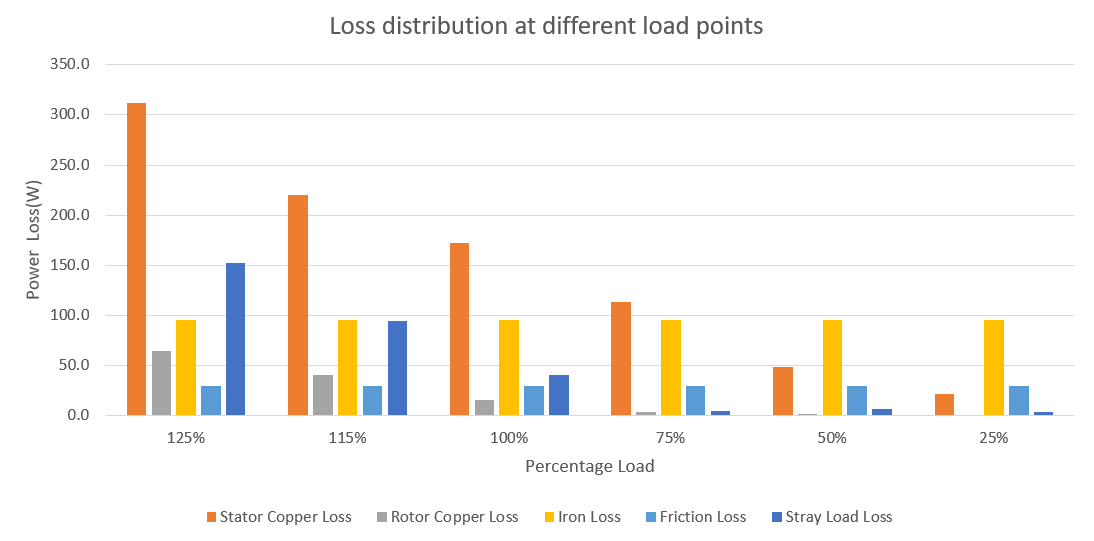
\includegraphics[width = 4.5in]{./Figures/MS/fig515.png}
		\rule{35em}{0.5pt}
	\caption{Bar graph for losses at different load points for 1.5 hp motor(method1)}
	\label{fig:Bar graph for losses at different load points for 1.5 hp motor(method1)} 
\end{figure}

\begin{figure}[hbtp!]
	\centering
		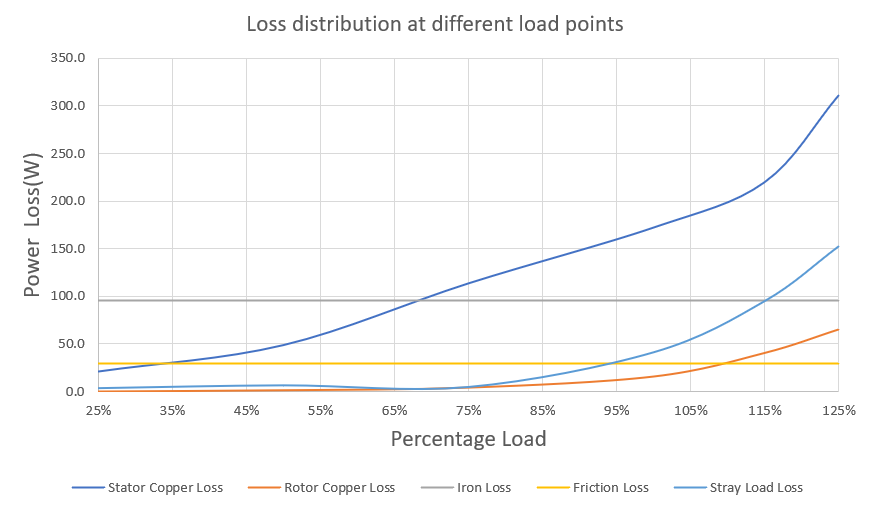
\includegraphics[width = 4.5in]{./Figures/MS/fig516.png}
		\rule{35em}{0.5pt}
	\caption{Line chart for losses at different load points for 1.5 hp motor(method1)}
	\label{fig:Line chart for losses at different load points for 1.5 hp motor(method1)} 
\end{figure}

\begin{figure}[hbtp!]
	\centering
		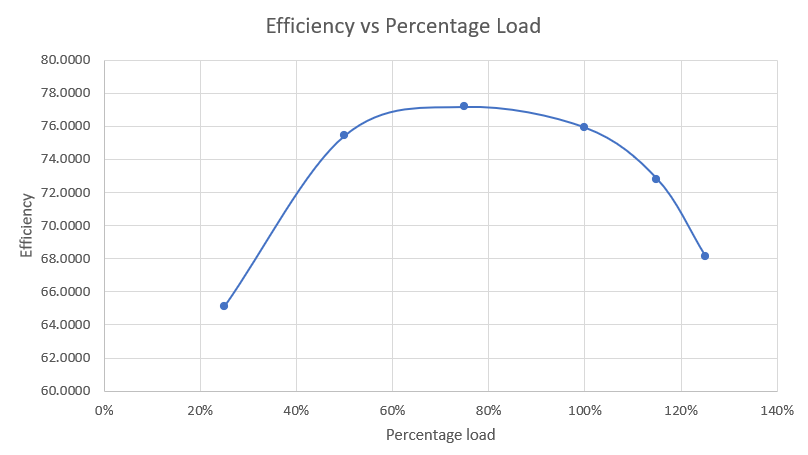
\includegraphics[width = 4.5in]{./Figures/MS/fig517.png}
		\rule{35em}{0.5pt}
	\caption{Percentage load vs efficiency for 1.5 hp motor(method1)}
	\label{fig:Percentage load vs efficiency for 1.5 hp motor(method1)} 
\end{figure}

\begin{figure}[hbtp!]
	\centering
		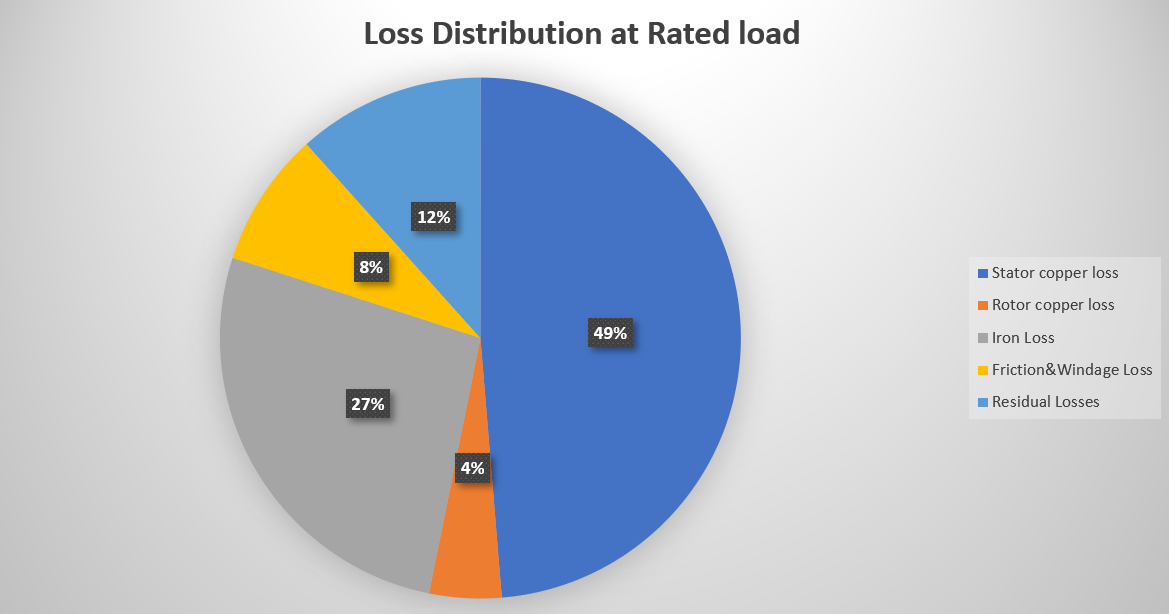
\includegraphics[width = 4.5in]{./Figures/MS/fig518.png}
		\rule{35em}{0.5pt}
	\caption{Pie chart for loss distribution at rated load for 1.5 hp motor(method1)}
	\label{fig:Pie chart for loss distribution at rated load for 1.5 hp motor(method1)} 
\end{figure}

\clearpage
\subsection{Method 2}
\subsubsection{Rated Load Test}
Following table shows the test results:
\begin{table}[hbtp!]
\begin{tabular}{
    >{\columncolor[HTML]{9B9B9B}}l llll}
    \cellcolor[HTML]{656565}{\color[HTML]{000000} Name} & \cellcolor[HTML]{656565}Symbol            & \cellcolor[HTML]{656565}Value     & \cellcolor[HTML]{656565}Unit &  \\
    {\color[HTML]{000000} Current}                      & I                                         & 4.7048                            & A                            &  \\
    {\color[HTML]{000000} Input   Power}                & \cellcolor[HTML]{F2F2F2}P1                & \cellcolor[HTML]{F2F2F2}978.13    & \cellcolor[HTML]{F2F2F2}W    &  \\
    {\color[HTML]{000000} Speed}                        & w                                         & 303.6252                          & rad/s                        &  \\
    {\color[HTML]{000000} Torque}                       & \cellcolor[HTML]{F2F2F2}T                 & \cellcolor[HTML]{F2F2F2}2.4569    & \cellcolor[HTML]{F2F2F2}Nm   &  \\
    {\color[HTML]{000000} stator   resistance}          & R1                                        & 3.9                               & ohm                          &  \\
    {\color[HTML]{000000} slip}                         & \cellcolor[HTML]{F2F2F2}s                 & \cellcolor[HTML]{F2F2F2}0.0330    & \cellcolor[HTML]{F2F2F2}     &  \\
    {\color[HTML]{000000} Output   Power}               & P2                                        & 745.97675                         & W                            &  \\
    efficiency                                          & \cellcolor[HTML]{F2F2F2}P2/P1*100         & \cellcolor[HTML]{F2F2F2}76.26560  & \cellcolor[HTML]{F2F2F2}\%   &  \\
    Actual   losses                                     & P1-P2                                     & 232.15325                         & W                            &  \\
    Stator   Copper Loss                                & \cellcolor[HTML]{F2F2F2}Ps                & \cellcolor[HTML]{F2F2F2}86.32706  & \cellcolor[HTML]{F2F2F2}W    &  \\
    Rotor   Copper Loss                                 & Pr                                        & 26.55133                          & W                            &  \\
    Temp   correction factor                            & \cellcolor[HTML]{F2F2F2}k                 & \cellcolor[HTML]{F2F2F2}0.99631   & \cellcolor[HTML]{F2F2F2}     &  \\
    Temp corrected   slip                               & sc                                        & 0.03292                           &                              &  \\
    Temp   corrected Stator copper loss                 & \cellcolor[HTML]{F2F2F2}Ps,c              & \cellcolor[HTML]{F2F2F2}86.32706  & \cellcolor[HTML]{F2F2F2}W    &  \\
    Temp   corrected Rotor copper loss                  & Pr,c                                      & 26.45339                          & W                            &  \\
    Iron Loss                                           & \cellcolor[HTML]{F2F2F2}Pfe               & \cellcolor[HTML]{F2F2F2}88.20973  & \cellcolor[HTML]{F2F2F2}W    &  \\
    Friction\&Windage   Loss                            & Pfw                                       & 10.22740                          & W                            &  \\
    Calculated   Losses                                 & \cellcolor[HTML]{F2F2F2}Ps,c+Pr,c+Pfe+Pfw & \cellcolor[HTML]{F2F2F2}211.21757 & \cellcolor[HTML]{F2F2F2}W    &  \\
    Residual   Losses                                   & P\_Lr                                     & 20.93567                          & W                            & 
\end{tabular}
\end{table}

\subsubsection{Load curve test}
Following table shows the test results:
\begin{table}[hbtp!]
\begin{tabular}{
    >{\columncolor[HTML]{9B9B9B}}l llllll}
    \cellcolor[HTML]{656565}Load points & \cellcolor[HTML]{656565}125\% & \cellcolor[HTML]{656565}115\% & \cellcolor[HTML]{656565}100\% & \cellcolor[HTML]{656565}75\% & \cellcolor[HTML]{656565}50\% & \cellcolor[HTML]{656565}25\% \\
    Input Power                         & 2051.5                        & 1766.5                        & 1472.4                        & 1086.52                      & 740.89                       & 430.66                       \\
    Current                             & 9.4328                        & 7.9311                        & 7.0218                        & 5.7034                       & 3.7456                       & 2.4664                       \\
    Speed                               & 301.8                         & 305.2142                      & 309.8572                      & 312.4219                     & 313.1297                     & 313.6544                     \\
    Torque                              & 4.634621272                   & 4.216291378                   & 3.6111                        & 2.686156124                  & 1.78686                      & 0.889113                     \\
    slip                                & 0.0389                        & 0.0280                        & 0.0132                        & 0.0050                       & 0.0028                       & 0.0011                       \\
    Output Power                        & 1398.7287                     & 1286.8720                     & 1118.9253                     & 839.2140                     & 559.5189                     & 278.8743                     \\
    Actual Losses                       & 652.7713                      & 479.6280                      & 353.4747                      & 247.3060                     & 181.3711                     & 151.7857                     \\
    Efficiency                          & 68.1808                       & 72.8487                       & 75.9933                       & 77.2387                      & 75.5198                      & 64.7551                      \\
    Stator Copper Loss                  & 311.4220                      & 220.1582                      & 172.5699                      & 113.8507                     & 49.1033                      & 21.2910                      \\
    Rotor Copper Loss                   & 63.9136                       & 40.6064                       & 15.8949                       & 4.4105                       & 1.6538                       & 0.3459                       \\
    Calculated Losses                   & 500.1115                      & 385.5406                      & 313.2407                      & 243.0372                     & 175.5331                     & 146.4128                     \\
    P\_lr                               & 152.6598                      & 94.0874                       & 40.2340                       & 4.2688                       & 5.8380                       & 5.3729                      
\end{tabular}
\end{table}

\subsubsection{No load test}
\begin{table}[hbtp!]
\begin{tabular}{llll}
    \rowcolor[HTML]{656565} 
    Name                                                              & Symbol  & Value    & Unit  \\
    \cellcolor[HTML]{656565}Voltage                                 & V\_0    & 220      & V       \\
    \rowcolor[HTML]{F2F2F2} 
    \cellcolor[HTML]{656565}Current                                 & I\_0    & 1.5107   & A       \\
    \cellcolor[HTML]{656565}Input Power                             & P\_0    & 106.4249 & W       \\
    \rowcolor[HTML]{F2F2F2} 
    \cellcolor[HTML]{656565}Stator Copper Loss                      & P\_s\_0 & 7.9877   & W       \\
    \cellcolor[HTML]{656565}Speed at rated power                    & n\_rl   & 303.6252 & rad/s   \\
    \rowcolor[HTML]{F2F2F2} 
    \cellcolor[HTML]{656565}Torque Req. to rotate unenergized motor & T\_0    & 0.0307   & Nm      \\
    \cellcolor[HTML]{656565}Friction\&Windage Loss                  & P\_fw   & 10.2274  & W       \\
    \rowcolor[HTML]{F2F2F2} 
    \cellcolor[HTML]{656565}Iron Loss                               & P\_fe   & 88.2097  & W      
\end{tabular}
\end{table}

\begin{figure}[hbtp!]
	\centering
		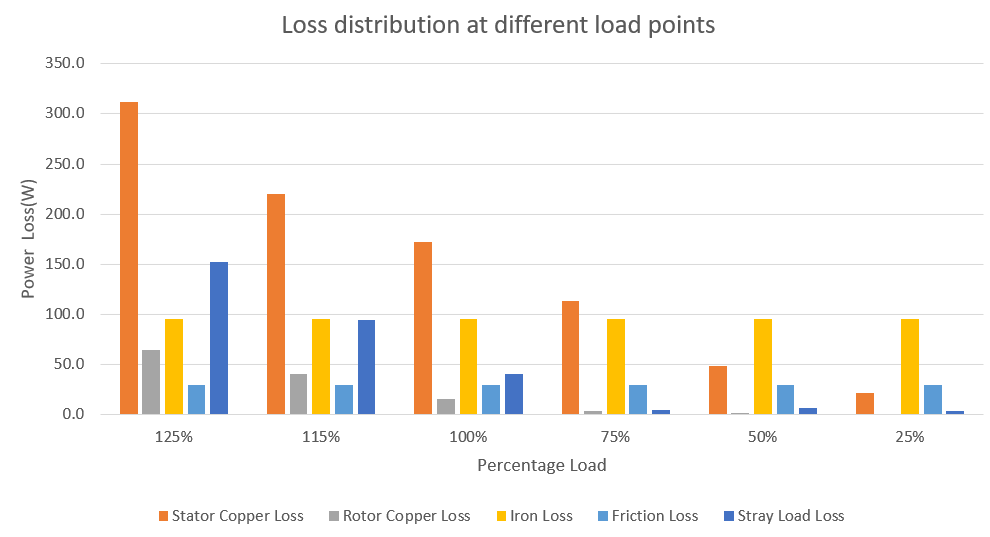
\includegraphics[width = 4.5in]{./Figures/MS/fig519.png}
		\rule{35em}{0.5pt}
	\caption{Bar graph for losses at different load points for 1.5 hp motor(method2)}
	\label{fig:Bar graph for losses at different load points for 1.5 hp motor(method2)} 
\end{figure}

\begin{figure}[hbtp!]
	\centering
		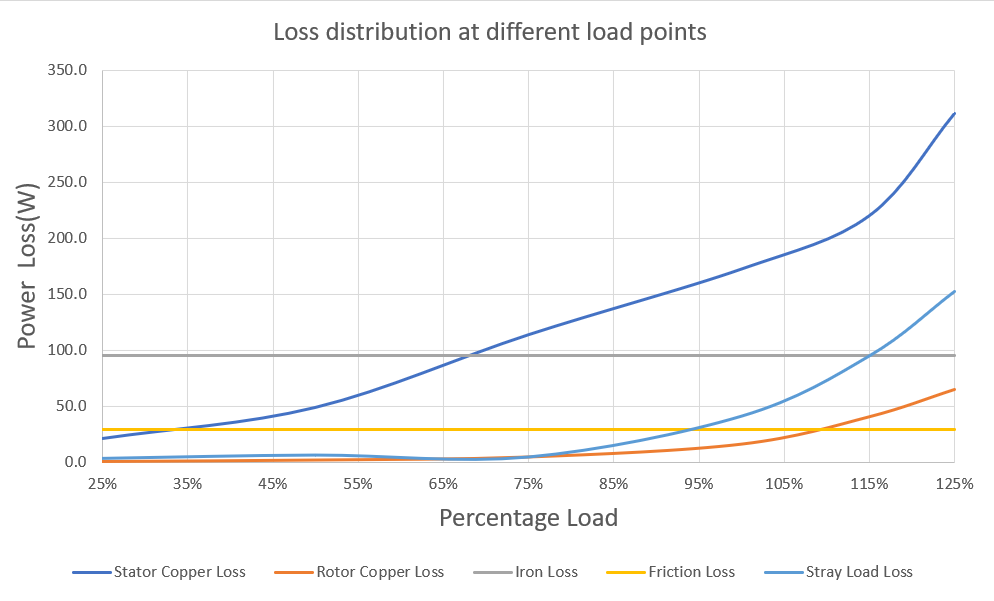
\includegraphics[width = 4.5in]{./Figures/MS/fig520.png}
		\rule{35em}{0.5pt}
	\caption{Line chart for losses at different load points for 1.5 hp motor(method2)}
	\label{fig:Line chart for losses at different load points for 1.5 hp motor(method2)} 
\end{figure}

\begin{figure}[hbtp!]
	\centering
		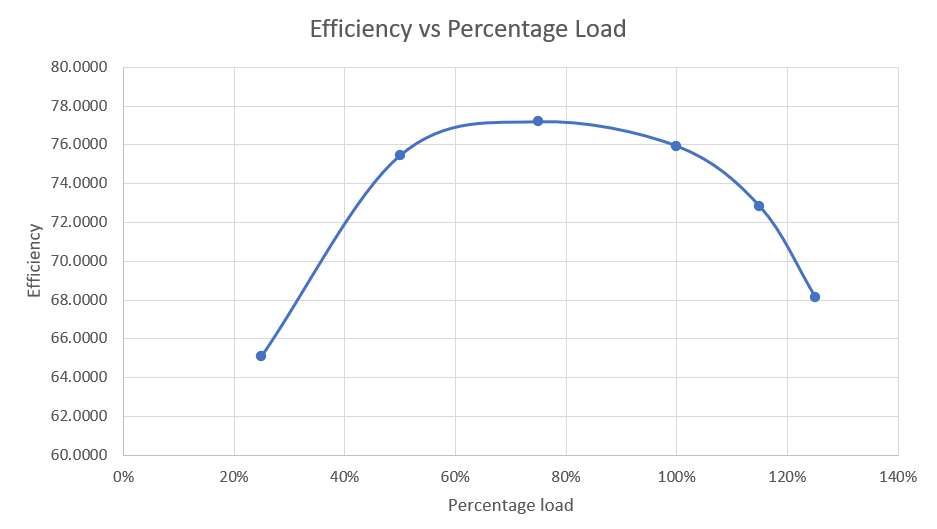
\includegraphics[width = 4.5in]{./Figures/MS/fig521.png}
		\rule{35em}{0.5pt}
	\caption{Percentage load vs efficiency for 1.5 hp motor(method2)}
	\label{fig:Percentage load vs efficiency for 1.5 hp motor(method2)} 
\end{figure}

\begin{figure}[hbtp!]
	\centering
		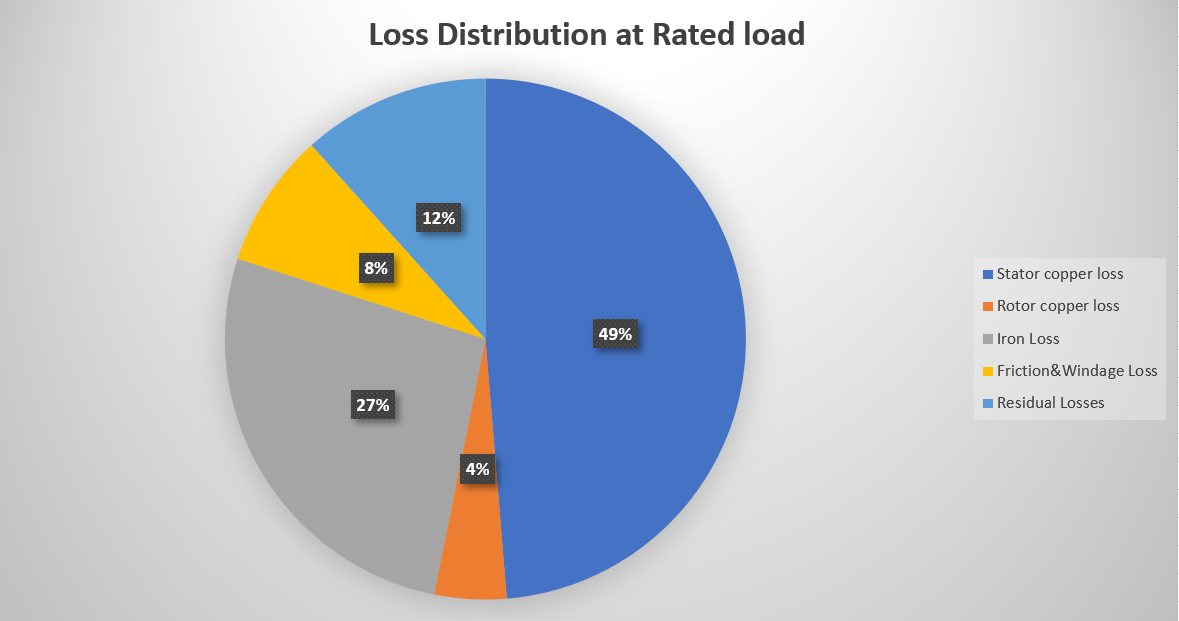
\includegraphics[width = 4.5in]{./Figures/MS/fig522.png}
		\rule{35em}{0.5pt}
	\caption{Pie chart for loss distribution at rated load for 1.5 hp motor(method2)}
	\label{fig:Pie chart for loss distribution at rated load for 1.5 hp motor(method2)} 
\end{figure}

\clearpage
\section{Concluding Remarks}
\begin{itemize}
    \item The algorithms applied and results of the simulation serve as a preliminary analysis for the formation of the actual hardware test benches. 
    \item By replacing the dynamometer with a pump and connecting pressure transducers and flow rate sensors, this setup can be extended to a testbench for pump testing according to ISO-9906
    \item Since the algorithm has shown to be working on multiple setups, hence it can be used to test other setups as well, if they will be able to work or not before building the actual setup. Once such setup tested was using a dc supply will a single-phase motor to apply the phenomenon of dc injection braking, which was not successful.
    \item This setup can also be used by students who are studying electric motors, so that their dependance on actual hardware for understanding the concepts of motors and measuring their parameters using tests is reduced.
\end{itemize}

